\documentclass[a4paper,12pt]{article}

% Encoding support.
\usepackage{ucs}
\usepackage[utf8x]{inputenc}
\usepackage[T2A]{fontenc}
\usepackage[russian]{babel}

\usepackage{graphicx}
\usepackage{listings}

\usepackage{amsmath, amsthm, amssymb}

%\usepackage{indentfirst}

\usepackage{hyperref}

\usepackage[final]{pdfpages}

\frenchspacing
\righthyphenmin=2

\textheight=24cm   
\textwidth=16cm    
\oddsidemargin=0pt 
\topmargin=-1.5cm  
\parindent=24pt    
\parskip=0pt       
\tolerance=2000

\title{Отчет по работе \\ по курсу <<Компьютерная алгебра>> }
\author{Смолов Виктор, Зенцев Фёдор, 4057/2}

\newcommand\Id[1]{\mathfrak{#1}}
\newcommand\BB[1]{\mathbb{#1}}



\begin{document}

\begin{titlepage}

\begin{center}

\large Санкт-Петербургский Государственный Политехнический Университет \\
Кафедра прикладной математики \\ [8.0cm]
\textbf{\textsc{ОТЧЕТ ПО ПРОИЗВОДСТВЕННОЙ ПРАКТИКЕ}}\\[3.0cm]

\begin{minipage}{0.4\textwidth}
\begin{flushleft} \large
  Выполнил студент гр. 3057/2: \\ [1.0cm]
  Руководитель:
\end{flushleft}
\end{minipage}
\begin{minipage}{0.4\textwidth}
\begin{flushright} \large
Зенцев Ф.К. \\ [1.0cm]
Павлов Д.А.
\end{flushright}
\end{minipage}

\vfill

\large Санкт-Петербург 2010



\end{center}
\end{titlepage}


\onecolumn

\setlength{\epigraphwidth}{8cm}

\begin{epigraphs}
  \qitem{Was hast du in Sommer gemacht? \\ Ich habe gespielt und gelacht}{\tiny{Из учебника по немецкому языку для начальной школы}}  \\ \\ 
  \qitem{There is an urban legend that Marvin Minsky assigned the problem of ``solving'' computer vision to a graduate
  student as a summer project. According to Minsky the legend is untrue - it was actually an undergraduate student.}
	 { \tiny{ \it{Artificial intelligence: A Modern Approach} \\ \textsc{Stuart J. Russell}}}
\end{epigraphs}  

\section*{Наcтоящее}

Студент Минского, как известно, свой летний проект не выполнил (что, впрочем, не помешало ему стать
Джеральдом Сассманом, профессором в MIT и автором замечательной книги и курса ``Структура и интерпретация
компьютерных программ'') - задачи распознавания изображений до сих пор остаются
одними из самых сложных задач искусственного интеллекта. Исторический опыт показал, что если ограничить задачу
компьютерного зрения определенным не слишком сложным (читай - не слишком обобщенным) классом объектов, то некоторого
успеха добиться всё-таки можно. Как распознавание текста и программа \begin{tt}Finereader\end{tt}, например. \\

\noindent
Летнюю производственную практику мне посчастливилось провести за решением нескольких задач, потребовавшихся
для проекта, посвященного распознаванию химических структур. В качестве введения проясню ценность и предназначение
такого проекта.\\

\noindent
Существует достаточно много различного рода программных продуктов разработанных для нужд специалистов в области химии:
редакторы молекул, системы поиска молекул в базах данных, системы моделирования химических реакций. Такое программное 
обеспечение работает с некоторым машинным представлением молекул.
В первом хемоинформатическом приближении молекулы,
химические структуры суть помеченные неориентированные графы, где метки вершин это названия атомов, а рёбер - различные
виды связей: двойная, тройная, стереосвязь. \\


\begin{figure}[h]
\centering
{\includegraphics[width=0.35\textwidth]{img/paracetomolum.pdf}}
{\includegraphics[width=0.25\textwidth]{img/aspirine.pdf}}
{\includegraphics[width=0.35\textwidth]{img/1.pdf}}
\caption{Парацетамол, аспирин и нарисованная автором молекула}
\end{figure}

\noindent Для машинного представления разработано несколько форматов файлов. Например \begin{tt}{MDL Molfile}\end{tt} или \begin{tt}Daylight SMILES\end{tt}.

\begin{figure}[h]
\centering
{\includegraphics[scale=0.8, clip, trim = 95mm 200mm 95mm 20mm]{img/benzene_smiles.pdf}}
{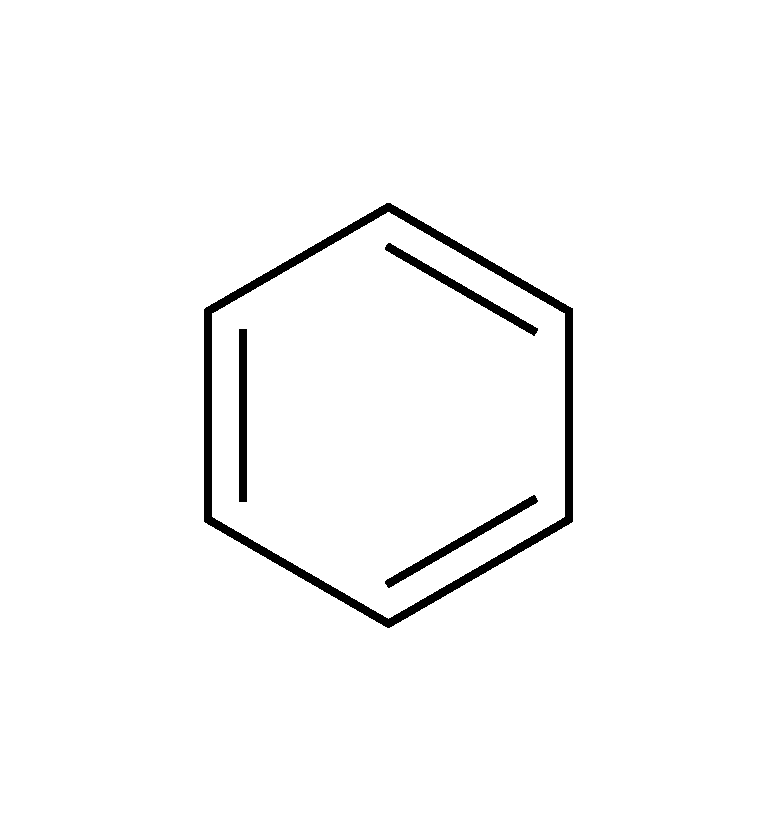
\includegraphics[scale=0.4, clip, trim = 25mm 10mm 25mm 10mm]{img/benzene.pdf}}
{\includegraphics[scale=0.6, clip, trim = 10mm 180mm 45mm 10mm]{img/benzene_molfile.pdf}}
\caption{Бензол в машинном представлении}
\end{figure}

\noindent Вообразим: специалист изучает статью по химии, в которой есть изображения молекул, и в некоторый момент у него возникает 
потребность загрузить какую-то молекулу и поработать с ней с помощью имеющегося у него инструментария. Да, конечно,
вполне возможно просто перерисовать молекулу, используя редактор и затем сохранить её. Но что, если нужных молекул много? 
Или, если молекула одна, но она достаточно большая и её перерисовка займет много времени? \\ 

\noindent 
Здесь и может вступить в игру распознавание изображений. Эта область искуственного интеллекта в некотором смысле ``обратна'' 
компьютерной графике. Если задача компьютерной графики визуализировать модель, в нашем случае отобразить молекулу, то задача 
распознавания изображений восстановить модель по картинке, то есть восстановить компьютерное представление молекулы. Или, 
если потребовать чуть большего, извлечь из статьи все молекулы. О более глобальном приложении распознавания химических структур 
можно прочесть в \cite{pavlov}.\\

\noindent
В рисунках молекул может присутствовать множество элементов, отображающих различные химические особенности соединений,
о распознавании двух из них я поведу речь далее. Надо сказать, что для распознавания не так уж важно, что элементы означают с точки 
зрения химии, куда важнее понять \emph{что} они являют собой на картинке, почему люди легко осознают, что это тот или 
иной элемент. И попытаться научить тому же самому компьютер. 

\section*{Стереосвязи}

Как правило, обычную одинарную связь на рисунке молекулы изображают единичным отрезком. Однако порой важно знать расположение
отдельного атома относительно плоскости остальной молекулы, т.е. находится ли атом, или, может быть, часть молекулы, выше или ниже.
Важность (как оказалось, исключительная важность в контексте фармакологии, см. \cite{chirality}) отображения такого свойства 
связана с такими понятиями как \emph{хиральность}, \emph{энантиомеры}, \emph{стереохимия}. Элементы это свойство отображающие - 
стереосвязи, будем называть их стерео-вниз (\emph{single down bond}) и стерео-вверх (\emph{single up bond}). В мои задачи 
входило распознавание стерео-вниз связей. \\

\noindent
Для начала пара слов о том, как вообще работает проект, в котором я участвовал. Распознавание представляет собой последовательное
извлечение из картинки различных элементов молекулы: букв, элементов графики. И затем некоторые результаты используются в последующих
этапах распознавания, например после того как были обработаны связи известна средняя длина связи на картинке и это помогало далее.
По определенным обстоятельствам извлечение стерео-вниз связей должно было идти первым этапом, следовательно о молекуле система в этот
момент ничего не знала. \\

\noindent
Исходя из наблюдений и согласуя их со стандартом отрисовки молекул (см. \cite{iupac}), я сформулировал критерий интересующих меня
элементов. Стерео-вниз связь - это набор из $k$, где $k \ge 3$, параллельных друг другу отрезков, следующих друг за другом
на примерно одинаковое расстояние. Критерий, как видно, конструктивен и из него был немедленно извлечен алгоритм.  

\begin{SCfigure}
\centering
{\includegraphics[scale=0.4, clip, trim = 15mm 10mm 15mm 10mm]{img/stereo.pdf}}
\caption{Закрашенный треугольник означает, что атом фтора находится ближе к обозревателю, это стерео-вверх связь. 
Треугольник, состоящий из параллельных отрезков говорит о том, что атом кислорода лежит за плоскостью картинки - стерео-вниз связь.}
\end{SCfigure} 

\begin{codebox}
  \Procname{\proc{FindSingleDownBonds}$(S)$}
  \li \Comment $Q$ - хранилище одиночных отрезков
  \li $Q = \varnothing$
  \li
  \li \Comment $S$ - хранилище сегментов картинки  
  \li \For $s \in S$ 	
  \li \Do \If \proc{IsSingleEdge}$(s)$
  \li   	\Then $Q \gets s$
  \li \End \End
  \li \Comment Все отрезки найдены, можно приступать к извлечению связей
  \li \For $a \in Q$
  \li \Do $L_{a} = \emptyset $ 
  \li \For $b \in Q, b \ne a$ 
  \li \Do \If $ a \parallel b $
  \li \Then $L_{a} \gets b$
  \li \End \End 
  \li \Comment Теперь в $L_{a}$ все отрезки параллельные $a$, осталось проверить расстояние
  \li \If \proc{CheckDistance}$(L_{a})$
  \li \Then \proc{AddSingleDownBond}$(L_{a})$
  \li \Comment Отрезки составили связь, больше они не понадобятся и будут только мешать
  \li \proc{DeleteSegments}$(L_{a})$
\end{codebox}

\noindent
Сегмент - компонент связности картинки. Ясно, что в $L_{a}$ может оказаться не одна связь, за этим следит функция \proc{CheckDistance}, выбирает
из набора параллельных отрезков, наборы с одинаковым расстояниями между соседними отрезками. Функция \proc{AddSingleDownBond} определяет
координаты начала и конца связи, а также её направление, затем добавляет в конструирующийся граф. Направление связи можно определить, узнав
какой из двух крайних отрезков длиннее. Однако встретились такие рисунки, где стерео-вниз связи были изображены отрезками по длине одинаковыми.
Казалось, что такой способ отрисовки вносит путаницу, на самом же деле это не так. Здесь пригодились некоторые сведения из химии: дело в том, что
существует конечный набор корректных конфигураций стереосвязей. Применение этих сведений требует знаний о том, какие атомы соединены стереосвязями,
какие еще связи у атома. Следовательно, этот этап отложен до момента, когда граф молекулы уже почти построен.  


\section*{Ароматичные кольца}

Существуют в химии понятия \emph{ароматичность}, ароматичная связь (\emph{aromatic bond}). Если в рисунке молекулы находится выпуклый 
многоугольник, целиком состоящий из ароматичных связей, то принято не изображать отдельно связи, а рисовать окружность внутри такого многоугольника.

\begin{figure}[h]
\centering
{\includegraphics[scale=0.4, clip, trim = 32mm 32mm 35mm 35mm]{img/rings.pdf}}
\caption{Ароматичные связи изображают двумя параллельным линиями: сплошной и пунктирной. Молекула справа получается из молекулы слева добавлением
недостающей ароматической связи.}
\end{figure}

\noindent
Возникает задача, которую сразу можно разбить на две подзадачи: необходимо найти на рисунке окружности, а затем пометить соответствующие связи, 
как ароматичные. Как и в случае со стереосвязями упомяну в какой момент должны распознаваться кольца: извлечение колец должно происходить после того, 
как из картинки уже были удалены все символьные данные и это хорошо, так как буквы \emph{O} могли бы ошибочно отсеятся. \\

\noindent
Для решения первой задачи я воспользовался тем, что в проекте уже успешно работало: распознаванием символов, которое основано на подсчете 
\emph{дескрипторов Фурье}.

\begin{codebox}
  \Procname{\proc{FindCircles}$(S)$}
  \li \Comment Пусть $I$ - пустая картинка, $Q$ - хранилище колец, а $S$ - хранилище сегментов картинки
  \li $I = \varnothing$
  \li $Q = \varnothing$
  \li \Comment Рисуем в $I$ окружность и считаем дескрипторы
  \li $\proc{PutCircle}(I)$
  \li $ FD_{c} = \proc{GetFourierDescriptors}(I)$
  \li \Comment Далее ищем похожие сегменты
  \li \For $s \in S$
  \li \Do $FD_{s} = \proc{GetFourierDescriptors}(s)$
  \li \If $FD_{s} = FD_{c}$
  \li \Then $Q \gets s$  
\end{codebox}

\noindent
Подсчет дескрипторов - процедура не слишком быстрая, и приведенный выше алгоритм можно ускорить, рассматривая только сегменты
с отношением ширины к высоте близким к единице, то есть квадратные сегменты. Теперь, когда все кольца извлечены, осталось подождать, пока
будет построен граф; связи, из которых состоят многоугольники, будут помечены как одинарные - внесём правки.

\begin{codebox}
  \Procname{$\proc{Aromatize}(G)$}
  \li \For $q \in Q$
  \li \Comment Для каждого кольца $q$ находим ближайшую к нему связь
  \li \Do $b = \proc{FindClosestBond}(q)$
  \li $begin\_vertex = b.end$
  \li $current\_vertex = begin\_vertex$
  \li $distance = \infty$
  \li \Comment Обходим многоугольник и помечаем связи 
  \li \Repeat 
  \li \For $v \in Adj(current\_vertex)$
  \li \Do \If $\proc{Distance}(Bond(v,current\_vertex), q) < distance $
  \li \Then $distance = \proc{Distance}(Bond(v,current\_vertex), q)$ 
  \li $next\_vertex = v $ \End \End
  \li $\proc{SetAromatic}(Bond(current\_vertex, next\_vertex))$
  \li $current\_vertex = next\_vertex$ \
  \li \Until $current\_vertex \ne begin\_vertex$
\end{codebox}

\noindent
Обход многоугольника осуществляется с естественной эвристикой: нет нужды далеко отходить от кольца. \\ 
\noindent
Подробнее о распознавании символов
и дескрипторах Фурье можно прочесть в \cite{smolov} и \cite{zahn}. Отмечу также, что для поиска окружностей существует известные методы, 
например преобразование Хафа (см. \cite{gonzalez}).

\section*{Будущее}

Не надо долго думать, чтобы понять как много вопросов и нерешенных сложных задач возникает в распознавании химических структур. Как
правильно разобрать картинку, в которой содержится не одна молекула, содержится реакция, таблица заместителей? Как вообще
найти изображение именно молекулы в статье? Как правильно обработать слипшиеся символы, слипшуюся связь и символ? Что касается задач изложенных
в этом отчете, то я бы сказал, что решены они были с точностью $\varepsilon$, как это обычно и бывает в распознавании изображений: остаются
кольца, у которых дескрипторы не совпадут (например на картинках плохого качества после сканирования), отрезки, которые не войдут в стереосвязи.

\onecolumn

\epigraph{Формат отчета свободный}{\tiny{профессор \tt{Штурц}}}

\section*{Замечания}

Проект собирался под операционные системы \begin{tt}Linux, Windows\end{tt} и \begin{tt}Mac OS X\end{tt} обеих, распространненных ныне разрядностей.
Разработка велась с помощью \begin{tt}Microsoft Visual Studio 2008\end{tt} и \begin{tt}NetBeans 6.8\end{tt} на языке \begin{tt}C++\end{tt}, 
для сборки была выбрана программа \begin{tt}scons,\end{tt} для контроля версий - \begin{tt}Subversion.\end{tt} Отчет был подготовлен в 
текстовом редакторе \begin{tt}vim\end{tt} с использованием \begin{tt}\LaTeX\end{tt}, иллюстрации в векторном виде подготовлены с помощью программ 
\begin{tt}dingo\end{tt} и \begin{tt}ketcher\end{tt}, в некоторых местах использовался \begin{tt}OpenOffice\end{tt}. Титульная страница 
взята из \cite[стр.26]{gluhov}. Все указанные программы, за исключением \begin{tt}Visual Studio\end{tt}, могут быть свободно загружены в интернете.

\begin{thebibliography}{9}

\bibitem{pavlov}
  Дмитрий Павлов,
  \emph{Навигация в мире органических соединений}.\\
  \url{http://shmat-razum.blogspot.com/2010/07/blog-post.html}

\bibitem{smolov}
  Виктор Смолов,
  \emph{Отчет по производственной практике}

\bibitem{chirality}
  \url{http://en.wikipedia.org/wiki/Stereochemistry}

\bibitem{iupac}
  \emph{Graphical Representation Standards For Chemical Structure Diagrams \\ (IUPAC Recommendations 2008)} \\
  \url{http://www.iupac.org/publications/pac/80/2/0277/}

\bibitem{gluhov}
  \emph{Правила оформления студенческих выпускных работ и отчетов. Положение.} 
  Под ред. В.В.Глухова.
  СПБ.:СПБГТУ, 1998

\bibitem{gonzalez}
  Gonzalez \& Woods,
  \emph{Digital Image Processing}

\bibitem{zahn}
  Charles T. Zahn \& Ralph Z. Roskies,
  \emph{Fourier Descriptors for Plane Closed Curves},
   IEEE Transactions on computers, Vol. c-21, No. 3, march 1972

\end{thebibliography}

\end{document}

